
%&LaTeX
\documentclass[12pt]{article}
\usepackage{latexsym}
\usepackage{epsf,amsmath}
\usepackage{graphicx}
\usepackage{multicol}
\usepackage{color}
\usepackage{txfonts}
\usepackage{bm}              % bold math and greek symbols
\usepackage{multicol} % allows some sections with multiple columns
\usepackage{wrapfig}  % allows text wrapped around figures
\usepackage{float}  % for figure positioning control

\setlength{\oddsidemargin}{-0.25in}
\setlength{\evensidemargin}{-0.25in}
\setlength{\topmargin}{-.75in}
\setlength{\headsep}{0in}
\setlength{\textwidth}{7in}
\setlength{\textheight}{9.8in}
\setlength{\parindent}{0in}
\renewcommand{\baselinestretch}{1.0}
\setlength{\parskip}{0.1in}

\usepackage{makeidx,afterpage,rotating,latexsym,psfrag,epsf,epsfig,amssymb,chicago,float,subfigure,color}
% package for neat insertion of hyperlinks
\usepackage[hidelinks]{hyperref}
\usepackage{xcolor}
\hypersetup{
    colorlinks,
    linkcolor={red!50!black},
    citecolor={blue!50!black},
    urlcolor={blue!80!black}
}
% easy use of \ceil and \floor:
\usepackage{mathtools}


\usepackage[colorinlistoftodos,linecolor=gray,backgroundcolor=white]{todonotes}

%\usepackage{footnote}
%\makesavenoteenv{tabular}
%\makesavenoteenv{table}



\DeclarePairedDelimiter\ceil{\lceil}{\rceil}
\DeclarePairedDelimiter\floor{\lfloor}{\rfloor}

%% Set Page Size etc,...
\setlength{\oddsidemargin}{8pt} \setlength{\evensidemargin}{-7pt}
\setlength{\hoffset}{0pt} \setlength{\voffset}{-36pt}
\setlength{\topmargin}{0pt} \setlength{\headheight}{10pt}
\setlength{\headsep}{15pt} \setlength{\footskip}{18pt}
\setlength{\columnsep}{20pt} \setlength{\paperheight}{846pt}
\setlength{\paperwidth}{594pt} \setlength{\textwidth}{449pt}
\setlength{\textheight}{681pt}


% my command definitions
% User-defined commands:
\newcommand{\ul}[1]{\underline{#1}}
\newcommand{\wh}[1]{\mbox{$\widehat{#1}$}}
\newcommand{\be}{\begin{eqnarray}}
\newcommand{\bes}{\begin{eqnarray*}}
\newcommand{\ee}{\end{eqnarray}}
\newcommand{\ees}{\end{eqnarray*}}
\newcommand{\bd}{\begin{description}}
\newcommand{\ed}{\end{description}}
\newcommand{\bi}{\begin{itemize}}
\newcommand{\ei}{\end{itemize}}
\newcommand{\ben}{\begin{enumerate}}
\newcommand{\een}{\end{enumerate}}
%\input{new_commands}


\newcommand{\gap}{\textcolor{white}}
\usepackage{ifthen}
\newboolean{includegapp}
\setboolean{includegapp}{true}
\newcommand{\gapp}[2]{\ifthenelse{#1}{#2}{}}
\newcommand{\garp}{\gapp{\boolean{includegapp}}}

\newboolean{includegappp}
\setboolean{includegappp}{false}
\newcommand{\gappp}[2]{\ifthenelse{#1}{#2}{}}
\newcommand{\gasp}{\gappp{\boolean{includegappp}}}

\newcommand{\mc}{0}  % Signals my copy for insertion of stuff
\newcommand{\workspace}[2]{\ifthenelse{\mc=1} {\parbox[b][#1][c]{15cm}{\tiny #2}} {\parbox[b][#1][c]{15cm}{}}}
\newcommand{\ql}{`}
\newcommand{\bn}{\begin{equation}}
\newcommand{\en}{\end{equation}}
\newcommand{\bna}{\begin{eqnarray}}
\newcommand{\ena}{\end{eqnarray}}
\newcommand{\und}{\underset}
\newcommand{\bnastar}{\begin{eqnarray*}}
\newcommand{\enastar}{\end{eqnarray*}}
\newcommand{\qql}{\textquotedblleft}
\newcommand{\qqr}{\textquotedblright}
\newcommand{\simdot}{\begin{array}{c} \vspace*{-20pt}\\
 . \vspace*{-7pt}\\ \sim \vspace*{-11pt}\\ .
\end{array}
}
\newcommand{\bs}[1]{\boldsymbol{#1}}
%\newcommand{\bv}{\footnotesize\begin{verbatim}}
%\newcommand{\ev}{\end{verbatim}\normalsize} % does not work because thinks this is verbatim text

\graphicspath{{./figures/}}

% the document


\pagenumbering{roman}
\setcounter{page}{1}


\includeonly{
maths,
distributions,
frequentist,
bayesian
}


\begin{document}

\abovedisplayskip 0.0in
\belowdisplayskip 0.0in

\centerline{\LARGE \bfseries Some Useful Maths and Stats} \vspace*{2 truemm}
\centerline{\Large \bfseries 2022/23}

\vspace*{10 truemm}

\begin{center}
David Borchers and Chris Sutherland
\end{center}

\vspace*{70 truemm}

\begin{center}
{\sc \Large University of St. Andrews }

~

\epsfxsize=0.5truein\epsffile{StAcrest.pdf}

~

{\sc \Large School of Mathematics and Statistics}
\end{center}

\newpage

\tableofcontents

\newpage

\pagenumbering{arabic}
\setcounter{page}{1}
\setcounter{equation}{1}

\hyphenpenalty=5000
\tolerance=1000

\section{Maths}

There is a lot of material on the web, and on YouTube in particular, that can help explain mathematical things. A favourite on differentiation, integration and related things is Grant Sanderson's \href{https://www.youtube.com/channel/UCYO_jab_esuFRV4b17AJtAw}{``Three Blue One Brown''} YouTube channel, which you will see that we link to at various points below.

\subsection{Derivatives}

Derivatives are just slopes of functions. There are some good videos on the meaning of derivatives and integrals \href{https://www.youtube.com/watch?v=WUvTyaaNkzM&list=PLZHQObOWTQDMsr9K-rj53DwVRMYO3t5Yr}{here}.

Table~\ref{tab:derivatives} shows some derivatives that are useful when manipulating probabilities and likelihood functions.

\begin{table}[ht]
\caption{Some derivative rules. Here $c$ is a constant, $f(\;)$, $g(\;)$ and $h(\;)$ are arbitrary functions, while $x$ and $y$ are variables.
\label{tab:derivatives}}
\begin{minipage}{\linewidth}
\begin{center}
\begin{tabular}{ll}
\hline
Function & Derivative ($f'=\frac{df}{dx}$) \\
\hline
$f(x)=c$ & $f'=0$ \\
$f(x)=x^y$ & $f'=yx^{y-1}$ \\
$f(x)=cg(x)$ & $f'=cg'$ \\
$f(x)=g(x)+h(x)$ & $f'=g'+h'$ \\
$f(x)=\log(x)$ & $f'=\frac{1}{x}$ \\
$f(x)=e^x$ & $f'=e^x$ \\
\hline
$f(x)=\log(x!)$ & $f'\approx\log(x)\footnote{This is an approximation that becomes exact as $x$ approaches $\infty$. (See below if you are unsure what $x!$ means.)}$ \\
\hline
\multicolumn{2}{c}{Chain rule} \\
General: $f(x)=h(g(x))$ & $f'=\frac{dh}{dg}\times\frac{dg}{dx}$ \\
Example 1: $f(x)=\log(g(x))$ & $f'=\frac{1}{g(x)}\times g'$ \\
Example 2: $f(x)=c\log(g(x))$ & $f'=\frac{c}{g(x)}\times g'$ \\
Example 3: $f(x)=e^{cx}$ & $f'= e^{cx}c$ \\
\hline
\end{tabular}
\end{center}
\end{minipage}
\end{table}


\subsection{Integrals}

Integration is just adding things up, but instead of adding discretely (first thing $+$ second thing $+$ third thing $+\cdots$), integration adds continuously. \href{https://www.mathsisfun.com/calculus/integration-introduction.html}{This website} describes the idea in simple terms, and Figure~\ref{fig:integral} illustrates the idea.

\begin{figure}[ht!]
\caption{\small The idea of an integral being the area under a curve, as the limit of a sum of more and more smaller and smaller things. In (a) the interval from -1 to 1.5 has been divided into 20 ``bins'' and the integral is approximated by the sum of the area of each histogram bar. In (b) it has been divided into 50 ``bins'' and we have not plotted the sides of the bins because that makes the plot messy. In (c) it has been divided into 1,000 bins and in this case the bin heights are indistinguishable from the smooth curve.}
\centering
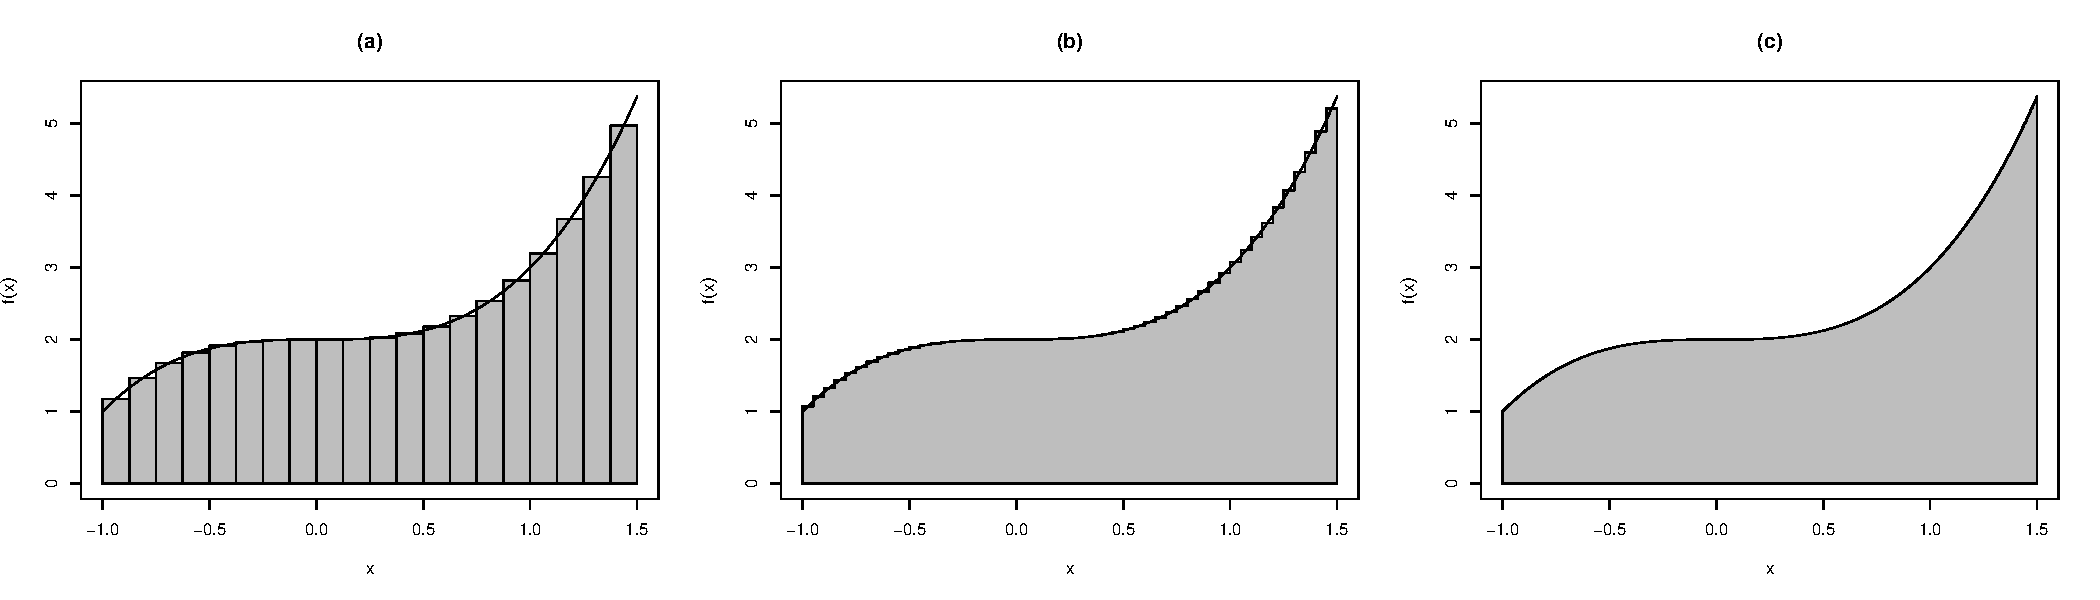
\includegraphics[width=\textwidth]{integralfigure.pdf}
\label{fig:integral}
\end{figure}

Figure~\ref{fig:integral} shows the function $f(x)=x^3+2$ plotted form $x=-1$ to $x=1.5$ as a smooth curve. The area under the curve is approximated by the sum
\be
\sum_{i=1}^K f(m_k)dx \nonumber
\ee
\noindent
where $m_k$ is the midpoint of the $k$th histogram bin, $K$ is the number of bins ($K=20$ in plot (a), $K=50$ in plot (a), $K=1,000$ in plot (c)), and $dx$ is the width of the bins (equal to $[1.5-(-1)]/K$). Notice that $f(m_k)dx$ is the area of the $k$th bin.

In the limit, as $K$ approaches infinity, this sum approaches the true area under the curve between $-1$ and $x=1.5$ (the integral of $x^3$ from -1 to 1.5), i.e., \\
\be
\lim_{K\rightarrow\infty}\sum_{i=1}^K f(m_k)\,dx&= &\int_{-1}^{1.5}f(x)\,dx. \nonumber
\ee

Integrals can be interpreted as \textbf{areas} under curves when integrating in one dimension (as in Figure~\ref{fig:integral}), and as \textbf{volumes} under surfaces when integrating in two dimensions.

\subsubsection{Integral examples}

A typical integral in statistics is the integral under a probability density function (PDF). This area is a probability. For example, the integral from $-\infty$ to $x$ of a the PDF of a standard nomal distribution is the \textbf{probability} that a standard normal random variable is less than or equal to $x$. \href{https://www.youtube.com/watch?v=ZA4JkHKZM50}{Here} is a video that explains how and why areas under PDFs are probabilities.

A different kind of integral that is common in statistical ecology is the integral under an animal density surface. A density surface quantifies the expected number of animals per unit area at any point. Remembering that an integral is just a sum of lots of heights multiplied by tiny widths in one dimenson, or heights multiplied by tiny \textit{areas} in two dimensions, the integral (volume) under the density surface over some region is the expected \textbf{number} of animals in the region (density in each tiny region multiplied by the area of the tiny region, gives the expected number in the tiny region). 

%Often we deal with estimated \textit{expected} density surfaces, and in this case the integral is the \textit{expected number} of animals.

\subsubsection{Computing integrals}

Mathematicians have worked out methods of obtaining formulae for the integrals of many functions. For example, the integral in Figure~\ref{fig:integral} is ($x^4/4+2x$ evaluated at $x=1.5$), minus ($x^4/4+2x$ evaluated at $x=-1$), i.e. $[1.5^4/4+2\times 1.5] - [(-1)^4/4+2\times(-1)] = 6.6.015625$.

The approximations calculated using sums with $K=20$, $K=50$ and $K=1,000$ are 6.013184, 6.015234, and 6.015624, respectively, i.e., they are incorrect by 0.04\%, 0.006\% and 0.00002\%.

It is frequently not possible to obtain formulae for the integrals of functions used in statistical ecology, and we frequently approximate them using sums similar to those shown above (or more sophisticated sums that give better approximations). %When \texttt{R} functions calculate integrals, they invariably used this kind of approximation.


\subsection{Logs}

Here are reminders of equalities involving logs of functions. These are the main ones you will need for routine manipulations of probabilities and likelihood functions.

\be
\log(xy)&=&\log(x)+\log(y) \nonumber \\
\log(x/y)&=&\log(x)-\log(y) \nonumber \\
\log(x^y)&=&y\log(x) \nonumber \\
\ee

Note: We use the ``natural log'' pretty much exclusively. This is log to the base $e$. It is often written as $ln$ rather that $\log$, but we will generally just use $\log$, in part because the \verb|R| has a function \verb|log()| that returns the natural log. 

But what is $e$? It is not crucial that you know what it is, but if you are interested, there are neat explanations \href{https://www.youtube.com/watch?v=AuA2EAgAegE}{here} and \href{https://www.youtube.com/watch?v=m2MIpDrF7Es&t=16s}{here}.

\subsection{Exponentials}

Here are reminders of equalities involving exponentials of functions. These are the main ones you will need for routine manipulations of probabilities and likelihood functions. (Note $e^x$ and $\exp(x)$ are the same thing.)

\be
\exp(x+y)&=&\exp(x)\times\exp(y) \nonumber \\
\exp(x-y)&=&\frac{\exp(x)}{\exp(y)} \nonumber \\
y\exp(x)&=&\exp\{\log(y)\}\times\exp(x)\;=\;\exp\{\log(y) + x\} \nonumber \\
\ee

\subsection{Factorials}

The factorial of an integer is the product of all integers from 1 up to the numebr in question. They are written by writing the number follow by an exclamation mark. So $1!=1$, $2!=1\times 2 = 2$, $3!=1\times 2\times 3 = 6$, $3!=1\times 2\times 3\times 4 = 24$, etc., and $n!=1\times 2\times\ldots\times n$. By convention, $0!=1$.

This $N\choose n$ is read as ``$N$ choose $n$'' and is the number of ways that you can choose $n$ items from $N$ available items (choosing each item at most once). It involves the product and ratio of factorials, thus:

\be
{N\choose n}&=&\frac{N!}{n!(N-n)!}.
\ee

\section{Statistical Modelling Basics}

Statistical modelling is the process of constructing mathematical models for data that arise from random processes. Statistical inference involves using these models to infer things about the generating processes. 

%Figure 9 illustrates this. Statistical modelling is required whenever we want to understand how data, ${\bf y}$ are generated by a stochastic process (i.e. a process involving randomness). It involves proposing a statistical model to explain how the data are generated, i.e. how the data arise from the parameters $\bm{\gamma}$ of the process that we know, the explanatory variables ${\bf x}$ that we know, and possibly some parameters $\bm{\theta}$ that we don't know. If there are some parameters that we don't know and are interested in knowing, we can use the statistical model together with observed the data ${\bf y}$, to infer the values of the parameters that we don't know. This process is called statistical inference, and is the focus of most of the rest of this module.

%\begin{figure}[ht!]
%\caption{\small Schematic representation of statistical modelling. We propose a statistical model (a pdf or pmf) to explain how the data $y$ are generated, i.e. how the data arise from the parameters $\bm{\gamma}$  that we know, the explanatory variables $\bm{x}$ that we know, and the parameters $\bm{\theta}$ that we don't know. Then once we observe the data, we use this statistical model (in the form of a likelihood function) to infer the values of the parameters that we don't know.}
%\centering
%\includegraphics[width=0.9\textwidth]{StatmodFigure.pdf}
%\label{fig:StatmodFigure}
%\end{figure}

There are a number of ways of doing statistical inference. The two main ones go under the names of ``frequentist inference" (also called ``classical inference'') and ``Bayesian inference". %Here we focus mainly on the former, but if you aspire to do applied statistics you really need to be familiar with both methods of inference. \todo[inline]{David says: Chris, this stuff is from a module I developed on maximum likelihood infrence - maybe we should add some basic Bayesian stuff to this document to make it more general?}

Both Bayesian and frequentist methods are based on likelihood functions. So proposing an appropriate likelihood function is absolutely central to developing a statistical model and to doing statistical inference. It is what links the things we observe (which include some random deviations from what is expected) to the things that we want to find out about but can't observe. It is different from the kinds of equations you will have dealt with in maths courses in that it includes a mathematical expression of the \textit{randomness} in the process.

The likelihood function is a quantitative description of the process that (we postulate) generated the observed data. The first step in statistical inference is identifying or proposing a probability distribution (which specifies the form of the randomness in the process) that might plausibly have generated the data.


\subsection{Likelihood functions}

A likelihood function is an expression that quantifies the likelihood of getting the observations you got. It is just a probability distribution function (PDF - if your data are continuous) or probability mass function (PMF - if your data are discrete). It contains some unknown parameters $\bm{\theta}$ (the things you want to estimate). For the purposes of inference, we treat the data as known values (after you observe them, they are known) and the parameters $\bm{\theta}$ as the things that the likelihood function depends on (they are unknown). Before you observe data, you have an expression that tells you the probability of getting any particular dataset. After you observe the data, you can use this to evaluate how likely any particular parameter values ($\bm{\theta}$) were to have generated the dataset.

Formulating likelihoods is just a question of writing down a PMF or PDF for the data you observed. This can be harder than it sounds. (For brevity, we will use the term ``probability distribution'' or just ``distribution'' to refert to PMFs and PDFs.)

\subsection{Building blocks: probability distributions}

The first step in obtaining a suitable likelihood is identifying a suitable PDF or PMF for the data at hand, and a first step in doing this is asking yourself whether the response (the random variable you are modelling - typically on the $y$-axis of a plot) is a continuous random variable (can take on values on a real line, e.g. anything between $-\infty$ and $\infty$, or between $0$ and $\infty$, or between $0$ and $1$), or a discrete random variable (can take on only specific discrete values, e.g. integers, or non-negative integers, or only the value $0$ or the value $1$). If it is continuous, you want to consider only PDFs; if it is discrete, you want to consider only PMFs.

Figure~\ref{fig:distributions} shows some common distributions, together with some of the relationships between them. In this figure, $n$ indicates counts (a discrete random variable), $\delta$ is a binary (and so discrete) random variable (0 or 1) and other responses are continuous. Among the continuous random variables, $t$ represents waiting time when on the left of ``$\sim$''and the $t$-distribution when on the right of it. 

The Poisson distribution is the ``mirror image'' of the exponential in the sense that if events occur randomly at an average rate of $\lambda$ then the waiting time between events has an exponential distribution with parameter $\lambda$, while the number of events occurring in an interval of length 1 has a Poisson distribution with parameter $\lambda$ (and the number of events occurring in an interval of length $t$ has a Poisson distribution with parameter $\lambda t$). The exponential's currency is time-per-event, while the Poisson's currency is events-per-time.\\

\begin{figure}[ht!]
\caption{\small Some common probability density and probability mass functions and some of the relationships between them.}
\centering
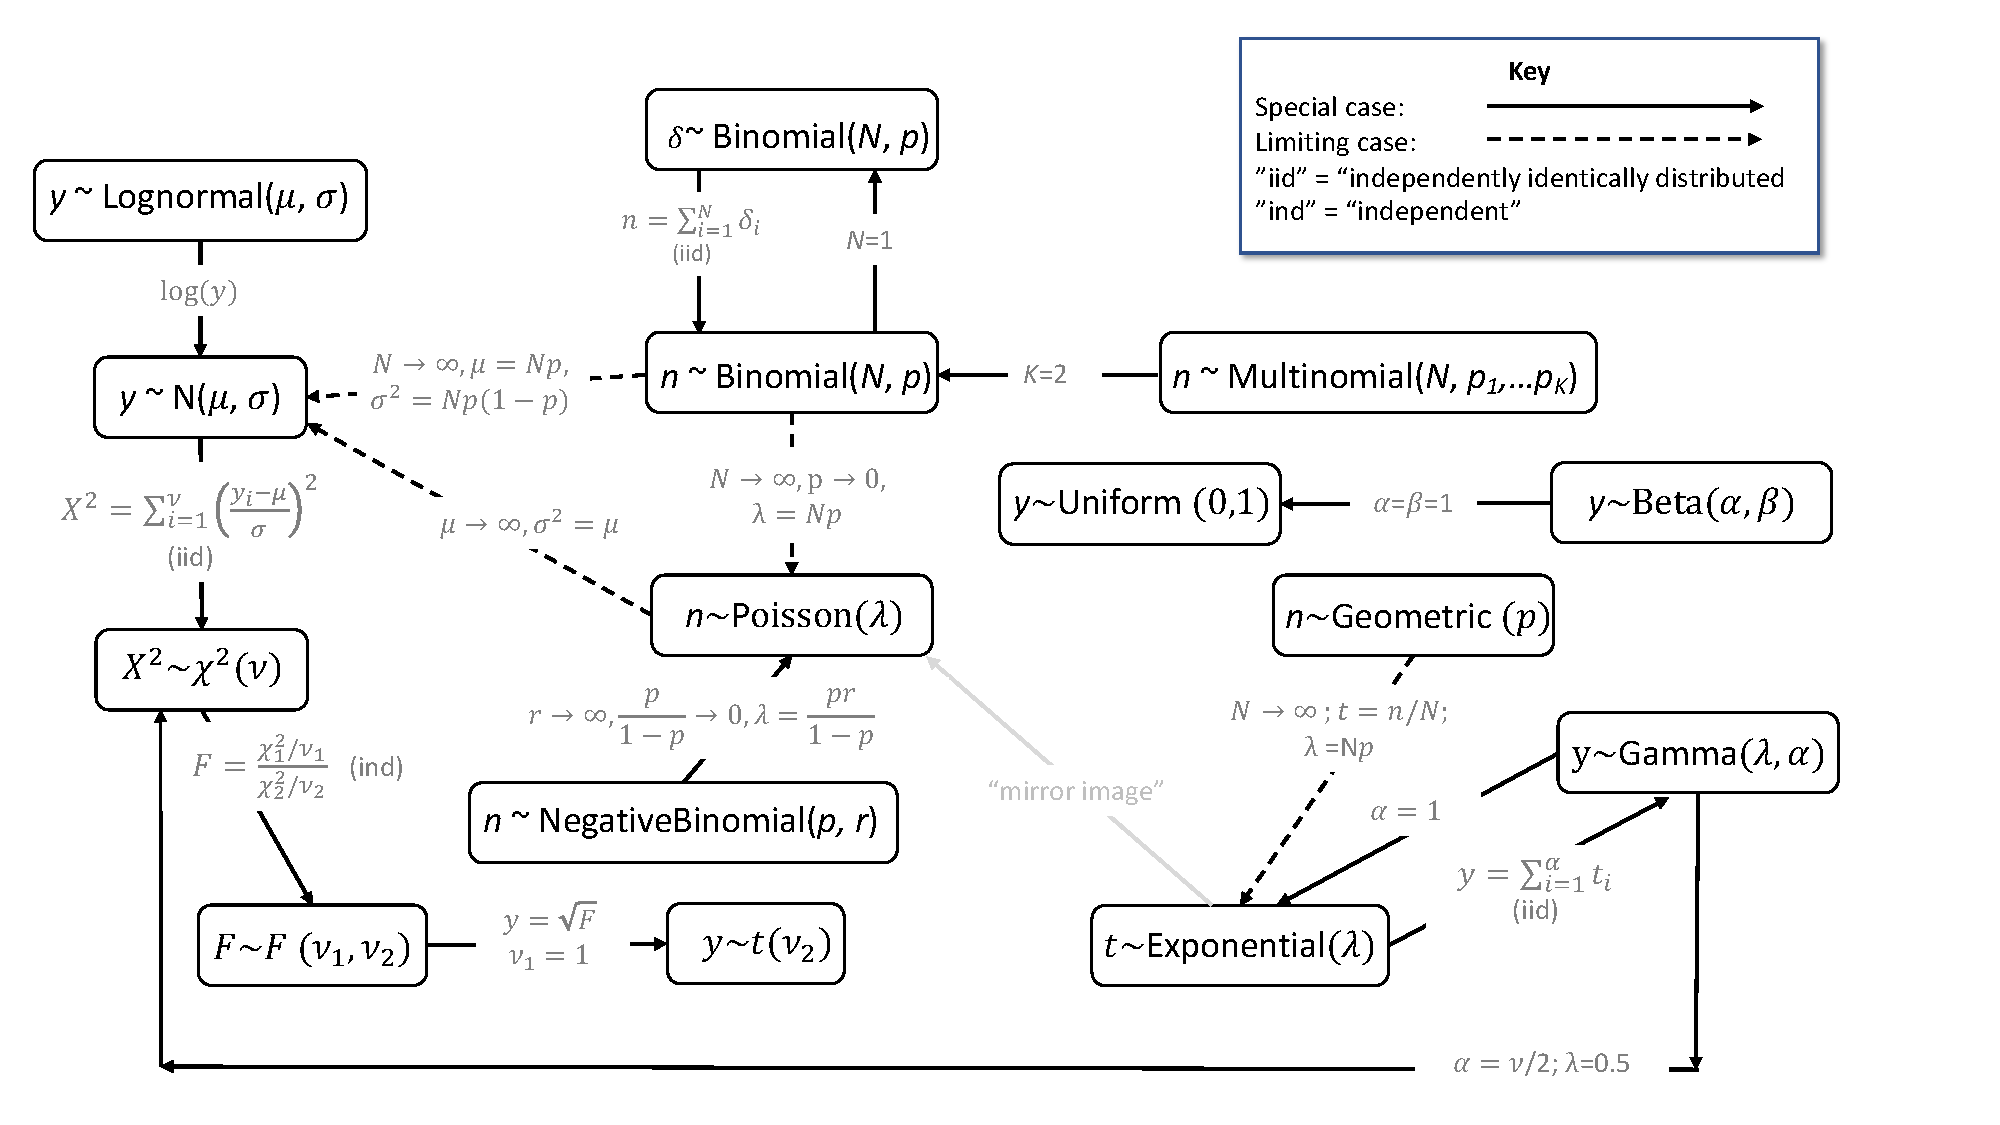
\includegraphics[width=1.1\textwidth]{distributions.pdf}
\label{fig:distributions}
\end{figure}


\begin{table}[ht]
\caption{Rough guide as to what each of the distributions in Figure~\ref{fig:distributions} is used for. The distributions in the top section of the table are PMFs for discrete random variables, while those in the bottom section are PDFs for continuous random variables.
\label{tab:distributions}}
\begin{center}
\begin{tabular}{rl}
\hline
PDF or PMF & Typical Use\\
\hline
Bernoulli & Used for binary data (e.g. success/failure, Yes/No).
\\
Binomial & Used for count data when there are a fixed number ($N$) of ``trials'', a \\
         & binary outcome for each trial, and the count is the number of ``successes''.
\\
Multinomial & Used for count data when there are a fixed number ($N$) of ``trials'' and \\
            & more than two possible kinds of outcome for each trial\\
Poisson & Used for count data when there is no limit on the size of the count, e.g. when \\
        & events occur at some  rate and we count the number of events in some interval.
\\
Negative Bionomial & Used as alternative to the Poisson distribution, when the variance \\
        & may be larger than the mean. 
\\
Geometric & Used for counts of number of events until the first ``success'', i.e. number of \\
          & events until some particular thing (a ``success'') occurs.
\\
\hline
Uniform & Used when all values in some interval are equally likely. \\
Exponential & Used for waiting time until some event. Similar to Geometric, but with \\
            & continuous wait time, instead of integer number of events. 
\\
Gamma & Generalisation of the Exponential to allow greater or lesser variance.
\\
Beta & Used for modelling the distribution of probabilities or proportions \\
     & (numbers between 0 and 1). \\
Normal & Used to model continuous random variables that can have values anywhere \\
       & on the real line (positive or negative). Use often justified by the Central \\
       & Limit Theorem.
\\
Lognormal & Used to model continuous random variables that can have values anywhere \\
       & on the real line greater than or equal to zero.
\\
$\chi^2$ & Used for squared standardised normal random variables.
\\
$F$ & Used for ratio of two independent Chi-squared random variables.
\\
$t$ & Special case of the F distribution; used for continuous random variables with \\
  & heavier tails than the Normal distribution.
\\
\hline
\end{tabular}
\end{center}
\label{default}
\end{table}

\clearpage

Consider Figure~\ref{fig:distributions} and Table~\ref{tab:distributions} to be the building blocks for likelihood functions. The first step in building an appropriate likelihood function for your data is identifying which of these blocks it is made out of.

\subsection{Suggest an appropriate distribution}

Here's an exercise in suggesting distributions appropriate for different kinds of data. For each of the scenarios below, propose at least one appropriate distribution.

\begin{enumerate}

\item A survey in which you count the number of daisies in randomly-chosen 1m$^2$ quadrats in a field.

\item A survey in which you count the number of females in a sample of $N$ animals.

\item A survey in which you are told only the proportion (not the numbers) of males in the catches of 10 fishing boats.

\item A survey in which you count the numbers of fish in each of 6 age classes in a catch of 100 fish.

\item A survey in which you record which of 100 ringed birds returns to its breeding site the following year.

\item A survey in which you count the number of attempts it takes a squirrel to get from the ground to a bird feeder hung high in a tree.

\item A survey in which you time how long it takes the squirrel to get to the bird feeder.

\item A survey in which you count the number of individuals that are photographed by a camera trap in a week.

\item A survey in which you observe the times between animals being photographed by a camera trap.

\item A survey in which you observe the weights of 50 praying mantis.

\item A survey in which you observe the mean weights of catches landed by 50 fishing boats.

\end{enumerate}
\subsection{Some useful facts about some distributions}

\textit{Hot tip: Wikipedia is an excellent source of information about probability distributions.}

\begin{enumerate}

\item \textbf{Mean-variance relationships} 

The relationship between the mean and the variance of many common probability distributions is ``hard-wired''. Some examples:

  \begin{enumerate}
  \item The mean of a Poisson distribution with parameter $\lambda$, is $\lambda$, and so is its variance.
%  \item The mean of a binomial distribution with parameters $N$ and $p$, is $Np$, and its variance is $Np(1-p)$.
  \item The mean of an exponential distribution with parameter $\lambda$, is $1/\lambda$, and its variance is $1/\lambda^2$.
  \item The mean of a geometric distribution with parameter $p$, is $1/p$, and its variance is $(1-p)/p^2$.
  \end{enumerate}
  
The normal distribution, with which most people are most familiar, is somewhat unusual in that its variance does not depend on its mean at all. This gives it additional flexibility. 

The gamma distribution is used to give the exponential distribution this kind of additional flexibility; by adding another parameter ($\alpha$) we get the flexibility to have the variance not depend on the mean.

In a similar way, the negative binomial distribution allows the variance of count random variables to be greater than the mean (unlike the case with Poisson counts), having an extra parameter ($r$) that controls the distribution's variance.

\item \textbf{``Thinned'' Poisson distribution}

Suppose that the number of things (e.g. animals in a population) is a Poisson random variable with parameter $\lambda$, and each of these things is detected independently with the same probability, $p$, then the number of \textit{detected} things is also a Poisson random variable, but with parameter $\lambda p$. The number of things is said to have been ``thinned'' by the detection probability $p$.

The Poisson distribution is unusual in this respect. It is generally the case that if the number of animals in a region has some given probability distribution, then the number of \textit{detected} animals will have an entirely different kind of distribution. But if the number of animals in a region has a Poisson distribution, then the number of \textit{detected} animals also has a Poisson distribution. This is a very convenient feature of the Poisson distribution.

\item \textbf{Poisson-Multinomial relationship}

Suppose the number of each of $K$ kinds of things is a Poisson random variable, with the $k$th kind having parameter $\lambda_k$, then if we ``condition on'' the total number of things, $N$, that were generated by these Poisson distributions (``conditioning on $N$'' means here ``once we know $N$''), then the number of things of each kind has a multinomial distribution with parameters $N$ and $p_1=\lambda_1/\sum_k\lambda_k,\ldots,p_k=\lambda_K/\sum_k\lambda_k$.

\item \textbf{The Poisson parameter depends on the interval}

If events occur independently at an average rate of $\lambda$ events per unit time, then the number of events in one time unit has a Poisson distribution with parameter (and mean) equal to $\lambda$, while the number of events in a time interval of length $T$ has a Poisson distribution with parameter (and mean) equal to $\lambda T$.

The same idea applies to events in space. If events occur independently at an average rate of $\lambda$ events per unit \textit{area} in space (e.g. if there are on average $\lambda$ animals per unit area, i.e., a density of $\lambda$ animals), then the number of events in a region with a surface \textit{area} of $A$ has a Poisson distribution with parameter (and mean) equal to $\lambda A$. And if each of these events (e.g. animals) is detected with probability $p$, then the number of \textit{detected} events (animals) has a Poisson distribution with parameter (and mean) equal to $p\lambda A$.


\end{enumerate}

\section{Frequentist Inference}

\subsection{Estimators and Sampling Distributions}

Estimators are just functions of random variables. (They are also statistics, because any function of random variablesis a statistic by definition.) Sampling distributions are the distributions of estimators. Usually estimators will be functions of more than one random variable. The canonical example of a sampling distribution is the distribution of the mean (of a sample of independent random variables), and in this case estimator (the sample mean) would typically be estimating the unknown population mean.

Estimators are typically written as the parameter they are estiamting, but with a ``hat''. So the estimators $\hat{\mu}$ and and $\hat{\sigma}$  below, would be estimators of the population mean $\mu$, and population standard error,  $\sigma$, respectively. 

\be
\hat{\mu}\;=\;\bar{y}&=&\frac{\sum_{i=1}^ny_i}{n} \\
\hat{\sigma}&=&\frac{\sum_{i=1}^n(y_i-\bar{y})^2}{(n-1)}
\ee

\noindent
where $y_1,\ldots,y_n$ is the observed data. Notice that $\hat{\mu}$ and $\hat{\sigma}$ are just functions of the random variables (the observed data) $y_1,\ldots,y_n$.

Figure~\ref{fig:samplingdbns} shows the sampling distribution of (a) the sample mean of a random variable $y$, (b) the standard deviation $\hat{\sigma}$, and (c) the \textit{geometric} mean $(\prod_{i=1}^ny_i)^{1/n}$, for samples of size $n=5$. 

\begin{figure}[ht!]
\caption{\small The sampling distribution of (a) the mean of a sample of $y$s, (b) the stanadard deviation $\hat{\sigma}$ of the sample, and (c) the geometric mean $(\prod_{i=1}^ny_i)^{1/n}$, for samples of size $n=5$.}
\centering
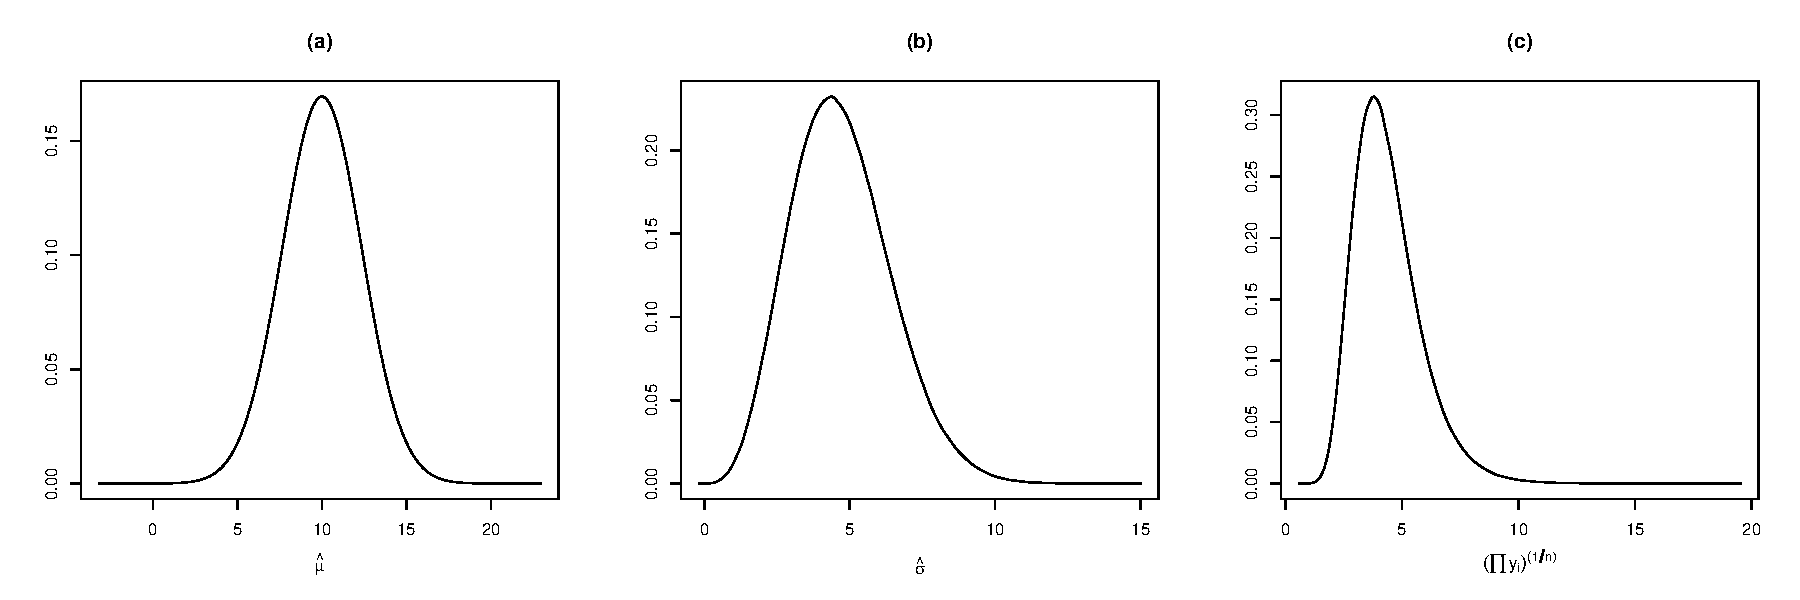
\includegraphics[width=0.9\textwidth]{samplingdbns.pdf}
\label{fig:samplingdbns}
\end{figure}

Sampling distributions depend on the statistic or estimator used (as is apparent from Figure~\ref{fig:samplingdbns}), and on the sample size (5 in this figure). The larger the sample size, the smaller the variance (width) of the sampling distribution.

We use the sampling distribution to get confidence intervals. For example, the point of the estimated sampling distribution of the mean that has 2.5\% of the density to the its left and the point that has 2.5\% to its right constitute the 95\% confidence bounds for the population mean.


\subsection{Estimator Properties}

The two main properties of estimators that we are most often interested in are their bias and their variance. Bias is just the difference between the expected value of the estimator (the mean of its sampling distribution) and the true value:

\be
\mbox{Bias}&=&E(\hat{\theta})-\theta,
\ee

\noindent
where $\hat{\theta}$ is the estimator of $\theta$. The variance of an estimator is the variance of its sampling distribution.

Note that individual estimates will be different from the true value of the parameter they are estimating, because estimators are random variables. The fact that a single estimate is  different from the true value does not mean that the estimator is biased, it is only when the \textit{expected value} of the estimator is different from the true value that we can say that the estimator is biased.

There are many possible estimators of any population parameter. For example, here is the maximum likelihood estimator (MLE) of $\sigma$, which is a little different from the usual estimator $\hat{\sigma}$:

\be
\tilde{\sigma}&=&\frac{\sum_{i=1}^n(y_i-\bar{y})^2}{n}.
\ee

We would like estimators to be unbiased and have low variance. One of the main reasons we use $\hat{\sigma}$ in preference to the MLE $\tilde{\sigma}$ is that $\hat{\sigma}$ is and unbiased estimator of $\sigma$, while $\tilde{\sigma}$ is biased by a factor of $n/(n-1)$.

\subsubsection{Expected values of nonlinear functions of estimators}

The expected value (mean) of a non-linear function of a random varible is \textbf{not} in general equal to the non-linear function of the expected value of the random variable. 

For example, suppose we know that $E(\hat{\theta})=\theta$, so that the random variable $\hat{\theta}$ is an unbiased estimator of $\theta$, but we are really interested in estimating $\exp(\theta)$, not $\theta$:

\be
\mbox{If}\;\;E\left(\hat{\theta}\right)=\theta&\mbox{then}&
E\left(e^{\hat{\theta}}\right)\neq e^{\theta}.
\ee

Because $\exp()$ is a nonlinear function, the expected value of $\exp(\hat{\theta})$ is \textit{not} $\exp(\theta)$, and so $\exp(\hat{\theta})$ is a \textit{biased} estimator of $\exp(\theta)$. This is an important fact that is often overlooked.

\subsection{Maximum Likelihood Estimation}

Suppose we want to estimate some parameter $\theta$ (e.g. the probability of detecting an animal) and we have some data $\bm{y}$ (e.g. the number of animals we detected). To make the example really simple, let's suppose that we also know the number of animals in the population, $N$, to be 100, and the number of detected animals is $y=10$. How would we estimate the detection probability $\theta$ by maximum likelihood?

Here is how we now proceed

\ben

\item \textbf{Get the likelihood function}: After referring to Table~\ref{tab:distributions}, we decide to model the data $y$ using a binomial distribution, and our likelihood function is therefore just the binomial distribution with some unknown $\theta$, evaluated at $y=10$ (with the detection, or ``success'' probability $\theta$ being unknown). We write it as $P(y=10;\theta)$, the ``$;\theta$'' being there just to make the dependence on the parameter $\theta$ explicit.  Because we know $y$, we think of this as a likelihod function that depends on the parameter $\theta$ and so write it as $L(\theta)$:

\be
P(y=10;\theta)\;=\;L(\theta)&=&{100\choose 10}\theta^{10}(1-\theta)^{100-10}.
\label{eq:binlik}
\ee

Figure~\ref{fig:thetalikelihood} shows the likelihood $L(\theta)$ for all values of $\theta$. 

\begin{figure}[ht!]
\caption{\small The likelihood function $L(\theta)$ for observed count $y=10$. The dashed red line shows where the maximum occurs.}
\centering
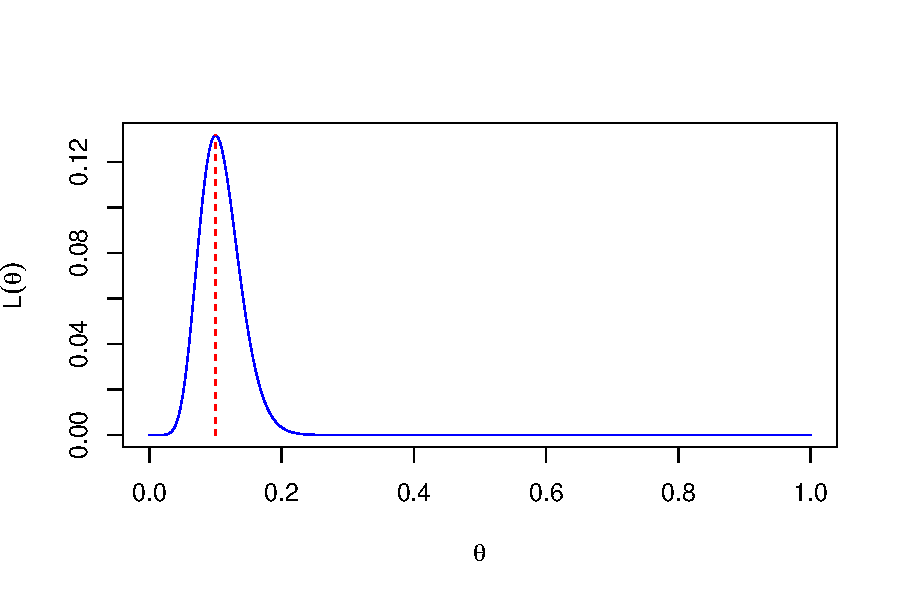
\includegraphics[width=0.55\textwidth]{thetalikelihoodmax.pdf}
\label{fig:thetalikelihoodmax}
\end{figure}

\item \textbf{Find the value of $\theta$ that maximises the likelihood function}. This is the maximum likelihood estimate (MLE). Finding it is just a question of finding the point at which the first derivative (the slope) of the likelihood function is zero and the second derviative (the rate of change of slope) is negative as you move from left to right. (Convince yourself that when the slope is zero, a negative second derivative corresponds to a maximum and a positive second derivative to a minimum of the function.)

Well, actually that is not what we do - we do that for the \textbf{log} of the likelihood function. Why? Because likelhood functions usually contain products of things and when you log the likelihood these become sums of things, and finding derivatives of sums is much easier than fiding derivatives of products. But are we sure that the maximum of the log-likelihood is at the same point as the maximum of the likelihood (I hear you ask)? Yes, because if any function increases, its log also increases, and if it decreases its log also decreases -- so the point at which the function is not increasing or decreasing (slope zero) is the point at which the log of the function is not increasing or decreasing.

By differntiating the log of Eqn~\eqref{eq:binlik} with respect to $\theta$ we find the slope of the log-likelihood, and by setting this slope equation to zero and solving for $\theta$ we find the MLE. (We should also calculate the second derivative and check that it is negative.) For this simple likelihood we can do this algebraically (try it yourself, using the relevant formulae for derivatives from the Maths section of these notes.) The maximum turns out to be at $\theta=y/N=10/100=0.1~$.

\begin{figure}[ht!]
\caption{\small The log-likelihood function $l(\theta)=\log\{L(\theta)\}$ for observed count $y=10$. The dashed red line shows where the maximum occurs.}
\centering
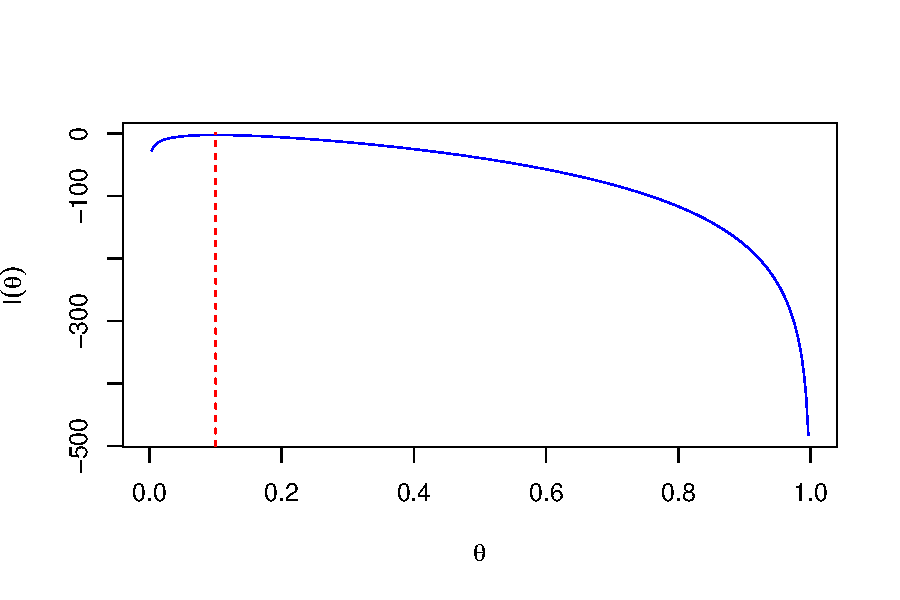
\includegraphics[width=0.55\textwidth]{thetaloglikelihoodmax.pdf}
\label{fig:thetaloglikelihoodmax}
\end{figure}

The maxima of the more complicated likelihood functions that we often have to deal with in realistically complex problems often cannot be found algebraically. In this case we find them by getting a computer to search (in an intelligent way) for the maximum. There are various algorothms for doing this, which we won't go into here.

\item \textbf{Find the sampling distribution of the MLE}. The MLE is just a function of the data (it is $\hat{\theta}=y/N$ in our simple example, where $y$ is the data) and so it has some sampling distribution. But what is its sampling distribution? For most MLEs, we don't actually know, so we usually either approximate the sampling distribution by simulating from our data or from our model using the MLE (bootstrapping), or we rely on powerful asymptotic results that give the sampling distribution of \textbf{any MLE} when sample size is ``large enough'' (strictly when it approaches $\infty$, but in practice for large samples). 

\een


\subsection{MLE Properties}

These are some key properties of MLEs:

\bi

\item MLEs are asymptotically unbiased (as sample size approaches $\infty$), but not necessarily unbiased for small sample sizes.

\item Asymptotically, MLEs have the smallest possible variance among all (asymptotically) unbiased estimators.

\item The sampling distribution of any MLE is (asymptotically, as sample size approaches $\infty$) normal, with mean equal to the true value of the parameter being estimated, and with variance equal to the inverse of the second derivative of the log-likelihood function (i.e., the inverse of the rate of change of the slope) at the MLE.

\item MLEs are ``invariant'', which means that the MLE of a function of an estimator is the function of the MLE. For example, we know that asymptotically, the sampling distribution of $\hat{\mu}$ is normal. Then (rather counter-intuitively) the sampling distributions of functions of $\hat{\mu}$ like $\exp(\hat{\mu})$ and $\sqrt{\hat{\mu}}$ are also asymptotically normally distributed, even though they are not normally distributed for finite sample size.
\ei


\section{Bayesian Inference}

Bayesian inference is based on Bayes' Theorem. This is a theorem whose utility is not restricted to Bayesian inference -- it is often used in Frequentist statistics too, but it is absolutely central to Bayesian inference. 

More generally, it is useful whenever you have the conditional probability of one thing (event B, say) happening, given that another (event A, say) has happened, and you want to find out what the conditional probability of A happening is, given that B has happened. 

That was a bit of a mouthfull, so let's look a an example to make it clearer. Suppose that you have an experssion for the probability of detecting an animal (event B, say), given that it is of sex male (event A, say) and you want to know what the probability of the animal being male (event A) is, given that you detected it (event B). To do this, you also need an expression for the unconditional probabilitiy of event A (i.e. of a randomly chosen animal in the population being male) and event B (i.e., of detecting any randomly chosen animal in the population). 

To understand Bayes' Theorem, you need to undestand what conditional probability is. You can find descriptions in many statistics textbooks and on the web. Here is one such explanation on \href{https://www.youtube.com/watch?v=ibINrxJLvlM}{YouTube}, and here is another explanation in the context of Bayes' theorem on the \href{https://www.youtube.com/watch?v=U_85TaXbeIo}{Three Blue One Brown} YouTube channel.

\subsection{Bayes Theorem}

Here it is:

\be
P(A|B)&=&\frac{P(B|A)P(A)}{P(B)}\\
\nonumber
\ee
\noindent

and here's a nice \href{https://www.youtube.com/watch?v=HZGCoVF3YvM}{visual explanation} of Bayes' Theorem (again from the Three Blue One Brown YouTube channel).

To continue the example about detecting animals of various sexes (and making it numerically similar to the example in the Three Blue One Brown video above), suppose that we have a weird population in which there is one male for every 20 females (i.e., $P(\mbox{male})=P(A)=1/21$), the probability that a randomly chosen animal is detected is $P(\mbox{detect})=P(B)=24/210$, and the probability of detecting a male is $P(\mbox{detect}|\mbox{male})=4/10$. Then the probability of a detected animal being male is 
\be
P(\mbox{male}|\mbox{detected})\;=\;P(A|B)
&=&
\frac{P(\mbox{detect}|\mbox{male})P(\mbox{male})}{P(\mbox{detect})} \nonumber \\
&=&
\frac{\frac{4}{10}\times\frac{1}{21}}{\frac{24}{210}}
\;=\;\frac{4}{24}. \\ \nonumber
\ee
(If you want to link this to the video: our males are the librarians in the video (the grey ones), our females are the farmers in the video (the green ones), and being detected in our example is like being ``a meek and tidy soul'' in the video.)

\subsection{Marginal probability and Joint probability}

The ``joint probability'' of A and B is the probability that both A and B occur and is written as $P(A\wedge B)$ or just $P(A,B)$. Note that

\be
P(A\wedge B)&=&P(A|B)P(B)\;=\;P(B|A)P(A).
\ee

\href{https://www.youtube.com/watch?v=CQS4xxz-2s4}{Here} is a decent YouTube video explaining marginal and joint probabilities.

If we knew $P(\mbox{detect}|\mbox{\textbf{fe}male})$, we could have worked out $P(\bm{detect})$ like this:

\be
P(\bm{detect})&=&P(\mbox{detect}|\mbox{male})P(\mbox{male}) + P(\mbox{detect}|\mbox{\textbf{fe}male})P(\mbox{\textbf{fe}male})
\ee

And in genenral, we can work out $P(B)$ by summing the joint probability of A and B, for all possible values of A:

\be
P(B)&=&\sum_{all\;possible\;A}P(B|A)P(A)
\ee

This is called the ``marginal probability'' of $B$. If A is a continuous random variable, we just integrate instead of summing:

\be
P(B)&=&\int_{-\infty}^{\infty}P(B|A)P(A)\;dA.
\ee



\subsection{Bayesian Estimation}

Lets look at the same example that we looked at when considering Frequentist inference. Here it is again: Suppose we want to estimate some parameter $\theta$ (e.g. the probability of detecting an animal) and we have some data $\bm{y}$ (e.g. the number of animals we detected). Recall that we made the example really simple  by supposing that we also know the number of animals in the population, $N$, to be 100, and the number of detected animals is $y=10$. How would we use Bayes' Theorem to estimate the detection probability $\theta$?

First, let's translate the problem into the notation that we used above:

\bi
\item A is $\theta$.
\item B is the data, $y$.
\item $P(B|A)$ is the probability of getting the data, $y$ (=10), given some value of the probability, $\theta$ (and the fact that we know $N=100$). We will consider all possibele values of $\theta$. This is the \textbf{likelihood function} -- see below.
\item $P(A)$ is our \textbf{prior} belief (before seeing the data) about what the detection probability $\theta$ is. We formulate this belief as a probability distribution, with high probability for values of $\theta$ that we think likely, and low probability for values we think unlikely -- see below.
\ei

Before we proceed, it is worth pointing out a fundamental philosophical difference between frequentist and Bayesian inference. Frequentist methods treat parameters (e.g. $\theta$) as \textbf{fixed values}, not random variables. We may not know their values, but the values are ``out there'' and fixed. Bayesian methods treat parameters as \textbf{random variables}, so from a Bayesian perspective $\theta$ is just another random variable. 

Here is how we now proceed:

\ben

\item \textbf{Get the likelihood function}: After referring to Table~\ref{tab:distributions}, we decide to model the data $y$ using a binomial distribution, and our likelihood function is therefore just the binomial distribution evaluated at $y=10$ (with the detection, or ``success'' probability $\theta$ being unknown). Because we know $y$, we think of this as a likelihod function that depends on the parameter $\theta$ and write it as $L(\theta)$. Note that, being Bayesian, we now treat $\theta$ as  random variable, and so think of the likelihood function as the conditional distribution of the data, given the random variable $\theta$:

\be
P(B|A)\;=\;P(y=10|\theta)\;=\;L(\theta)&=&{100\choose 10}\theta^{10}(1-\theta)^{100-10}.
\ee

Figure~\ref{fig:thetalikelihood} shows the likelihood $L(\theta)$ for all values of $\theta$. Its maximum occurs at the value $\theta=y/N=10/100=0.1$ (the frequentist maximum likelihood estimate).

\begin{figure}[ht!]
\caption{\small The likelihood function $L(\theta)$ for observed count $y=10$.}
\centering
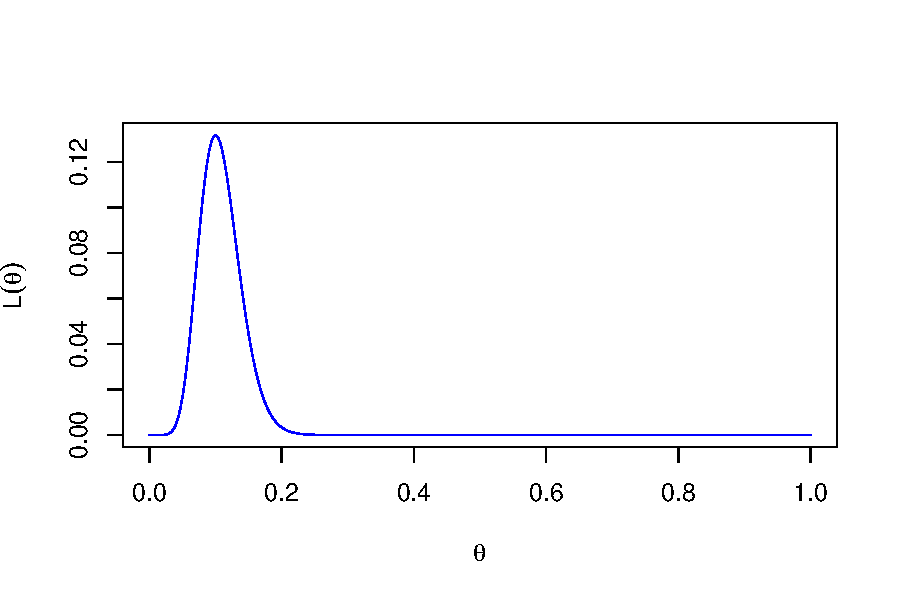
\includegraphics[width=0.55\textwidth]{thetalikelihood.pdf}
\label{fig:thetalikelihood}
\end{figure}

\item \textbf{The prior distribution}: Because $\theta$ is considered to be a random variable, we need to specify a distribution for it (this is called the ``prior'' distribution). After referring to Table~\ref{tab:distributions} again, and noting that $\theta$ is a probability, we decide to use a beta distribution for this. We choose its parameters $\alpha=3$ and $\beta=6$ to reflect our prior belief in what $\theta$ is, as shown in Figure~\ref{fig:thetaprior} (with $\theta=0.3$ being most likely and $\theta$ quite unlikely to be more than 0.6).

\begin{figure}[ht!]
\caption{\small Our prior distribution for $\theta$.}
\centering
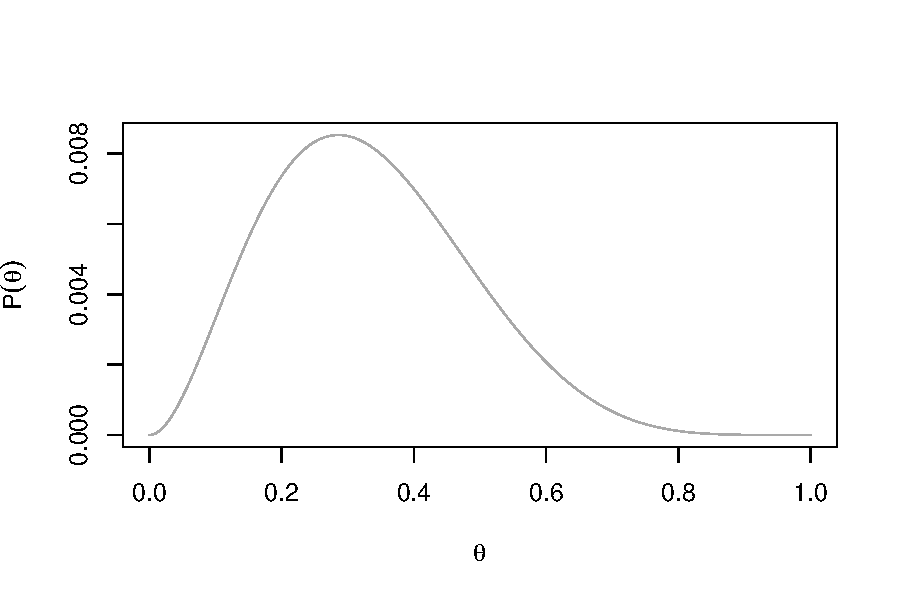
\includegraphics[width=0.55\textwidth]{thetaprior.pdf}
\label{fig:thetaprior}
\end{figure}

\item \textbf{The posterior distribution}: Armed with our likelihood $L(\theta)=P(y;\theta)$ and our prior distribution $P(\theta)$ for $\theta$, we use Bayes' Theorem to obtain the \textbf{posterior} distribution for $\theta$:

\be
P(A|B)&=&\frac{P(B|A)P(A)}{P(B)}\;=\;\frac{P(B|A)P(A)}{\int P(B|A)P(A)\;dA} \nonumber \\
P(\theta | y=10)&=&\frac{P(y=10|\theta)P(\theta)}{\int_0^1 P(y=10|\theta)P(\theta)\;d\theta}
\ee

Figure~\ref{fig:thetaposterior} shows the posterior distribution $P(\theta | y=10)$, overlaid on the prior and likelihood (scaled to integrate to 1 for comparability with the prior and posterior). You can see that the posterior distribution has been pulled a bit towards the prior (i.e. to the right), but not much and has a much narrower distribution than the prior. This indicates that the data contains a lot of information about $\theta$. If the data contained little information, the posterior would look more like the proir (the data will not have changed your prior belief much).

\begin{figure}[ht!]
\caption{\small The prior (grey dashed line), likelihood (blue dashed line) and posterior distribution (black line) of $\theta$.}
\centering
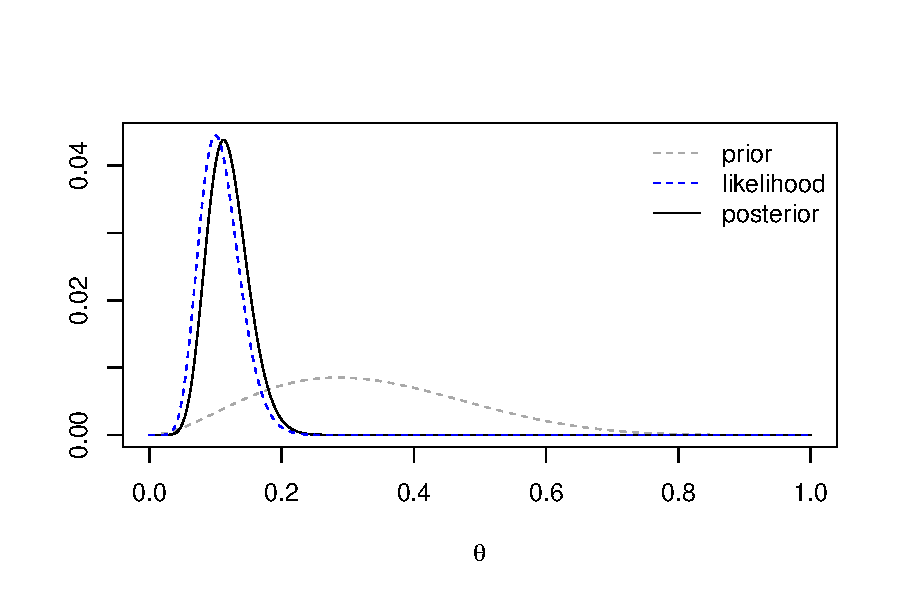
\includegraphics[width=0.7\textwidth]{thetaposterior.pdf}
\label{fig:thetaposterior}
\end{figure}
\nonumber

The posterior distribution (the black line in Figure~\ref{fig:thetaposterior}) is the Bayesian estimator for $\theta$. Notice that it is a distribution, not a single number. This is one of the attractive features of Bayesian estimators - they summarise in a probability distribution all that we know about the thing we are estimating, incuding the uncertainty and the most likely values. 

\een

In a similar way to the way that we get confidence intervals for parameters from the sampling distribution of a frequentist estimator, we get the Bayesian equivalent, ``credible intervals'' from the posterior distribution when doing Bayesian inference.

As a rule, if you use what is called an ``uninformative prior'' distribution (i.e. a prior distribution that equates to ``I have no prior knowledge of what $\theta$ is.''), then the value of $\theta$ at which the maximum of the Bayesian posterior distribution occurs, is the MLE of the parameter. (In our example, an uninformative prior would be one that assigns equal probability density to every value of $\theta$ between 0 and 1.)

Thought about in another way, the knowledge about $\theta$ that you encapsulate in the prior distribution, moves the most likely value for $\theta$ away from what it would be if you knew nothing about $\theta$ and only used the data $y_1,\ldots,n$ to inform you about it. And the MLE corresponds to the case in which you know nothing about $\theta$ before you take your sample.

\subsection{Bayesian Inference - an ecological perspective}

The above has shown how Bayesian inference works for a particular example, but the same ideas and methods apply whatever inference problem you are addressing. There are a growing number of ecological statisitcs texts that offer explanations of Bayesian inference from an ecological perspective. These resources are extrememly useful for reinforcing general statistical concepts by linking them to concrete and familiar ecological inference problems. 
The following two review papers describe why Bayesian inference should be of general interest to ecologists:

\begin{itemize}
\item Aaron, E. M. 2004. Bayesian inference in ecology. Ecology Letters 7:509–520. (\href{https://tinyurl.com/ya7d57qk}{PDF})
\item Clark, J. S. 2005. Why environmental scientists are becoming Bayesians. 8: 2-14 (\href{https://tinyurl.com/ycguf6w9}{PDF})
\end{itemize}

The following books are ``Bayesian statistics for ecologists`` reference books and the identified chapters are the ``Bayesian primer`` chapters:

\begin{itemize}
\item Kéry, M., 2010. Introduction to WinBUGS for ecologists: Bayesian approach to regression, ANOVA, mixed models and related analyses. Academic Press. Chapter 2 (\href{https://tinyurl.com/ycguf6w9}{PDF})
\item Kéry, M. and Schaub, M., 2011. Bayesian population analysis using WinBUGS: a hierarchical perspective. Academic Press. Chapter 2 (\href{https://tinyurl.com/ydyl9ont}{PDF})
\end{itemize}


\pagestyle{empty}

\clearpage
%\newpage

%\part{Tutorials}
%\include{tutorial1}

%\part{Tutorial Solutions}
%\include{tutorial1solns}

%\part{Project}
%\include{project}
%\include{projectsolns}

%\part{Additional Material}
%\include{AdditionalExamples}
%\include{AdditionalExamplesSolutions}

\end{document}


